
\documentclass[11pt]{article}
\usepackage[margin=1.0in]{geometry}

%\documentclass{pnas}
\usepackage{graphicx}
\usepackage{amsmath}
\usepackage{lscape}
\newcommand{\xline}[0]{\noindent\underline{\makebox[0.15cm][l]{}}}
\makeatletter
\def\hlinewd#1{%
	\noalign{\ifnum0=`}\fi\hrule \@height #1 \futurelet
	\reserved@a\@xhline}
\makeatother
\begin{document}
	
	
\title{The relationship between scaled selection coefficients and dN/dS}
	
\author{Stephanie J. Spielman\affil{1}{Department of Integrative Biology, Center for Computational Biology and Bioinformatics, and Institute of Cellular and Molecular Biology.
		The University of Texas at Austin, Austin, TX 78712, USA.} 
	\and
	Claus O. Wilke\affil{1}{}
}
	
%\contributor{Submitted to Proceedings of the National Academy of Sciences of the United States of America}
%\maketitle

%\begin{article}
		
\section*{Significance Statement} 
\textbf{NOT DONE, obviously, but maybe a general idea??} Competing modeling frameworks have been proposed to determine the strength of natural selection in protein-coding sequences. However, it remains unknown how distinct modeling frameworks relate to one another. Having a thorough understanding of the relationship among models is critical when selecting an appropriate framework to use. In addition, by elucidating the relationship among distinct frameworks, we can gain a deeper understanding of the individual models themselves. Here, we establish a formal mathematical relationship between distinct modeling frameworks, and we uncover important modeling properties which illuminate previously unrecognized limitations and behaviors inherent to each modeling framework.


\begin{abstract} 
%$dN/dS$ models have been developed to a high level of sophistication and are a staple of modern-day comparative sequence analysis.
The evolutionary rate ratio $dN/dS$, representing the ratio nonsynonymous to synonymous substitution rates, is widely used to infer the strength of natural selection in protein-coding sequences.  Recently, mutation-selection-balance (MutSel) models have become a popular alternative to the $dN/dS$ framework. MutSel models estimate scaled selection coefficients, indicating the selective response to particular codon and/or amino-acid changes, from phylogenetic data. However, it remains unknown how these two modeling frameworks relate to one another. Do $dN/dS$ estimates contain similar or distinct information from scaled selection coefficients? To answer this question, we have derived a formal mathematical relationship to calculate $dN/dS$ from scaled selection coefficients. We prove that, when synonymous changes are neutral, MutSel models strictly produce $dN/dS \leq 1$. Alternatively, if selection acts on synonymous changes, $dN/dS$ can readily be greater than 1, even though positive selection is not occurring. In addition, we used the relationship between models to examine the extent to which $dN/dS$ estimated using maximum likelihood (ML) agree with $dN/dS$ computed from selection coefficients. This analysis served as a novel and robust strategy for assessing the performance of ML $dN/dS$ inference frameworks. ML methods yielded biased $dN/dS$ estimates in the presence of mutational asymmetry, but this bias was ameliorated by fitting models which more closely matched the mechanistic process which generated the data. Strikingly, we found that the best-fitting model, based on AIC scores, was not necessarily the model with the least bias and highest precision for parameter estimates of interest. Therefore, we conclude that selecting models based solely on fit can be counterproductive and positively misleading. 
\end{abstract}
		
		

%\keywords{dN/dS | mutation-selection-balance models | scaled selection coefficients | Markov models of sequence evolution}


\section*{Introduction}
		
The oldest and most-widely used method to infer selection pressure in protein-coding genes calculates the evolutionary rate ratio $dN/dS$, which represents the ratio of non-synonymous to synonymous substitution rates. This metric indicates how quickly a protein's constituent amino acids change, relative to synonymous changes, and it is commonly used to identify protein sites that experience purifying selection ($dN/dS<1$), evolve neutrally ($dN/dS\approx1$), or experience positive, diversifying selection ($dN/dS>1$) \cite{NielsenYang1998, Yangetal2000, KosakovskyPondFrost2005b, Huelsenbecketal2006}. In phylogenetic contexts, $dN/dS$ is typically calculated using a maximum likelihood (ML) approach \cite{GoldmanYang1994,MuseGaut1994,NielsenYang1998,Yang2006}. ML methods assume an explicit continuous time Markov-process model of sequence evolution and yield maximum likelihood estimates (MLEs) of the parameter $\omega$, which represents the quantity $dN/dS$ (although we note that other styles of these models use separate parameters for nonsynonymous and synonymous substitution rates \cite{MuseGaut1994,KosakovskyPondMuse2005}). These $dN/dS$ models have become a staple of comparative sequence analysis since their introduction in the 1990s (see ref \cite{Anisimova2009} for a comprehensive review), and we will refer to them as $\omega$-based models throughout this paper.

A second class of Markov models, known as mutation-selection-balance (MutSel) models, are increasingly being viewed as a viable alternative to $\omega$-based models. While $\omega$-based models describe the how quickly a protein's constituent amino acids change, MutSel models assess the strength of natural selection operating on specific amino-acid or codon changes. The MutSel framework estimates site-specific scaled selection coefficients $S=2N_es$, which indicate the extent to which natural selection favors, or disfavors, particular codon or amino acid changes \cite{HalpernBruno1998,YangNielsen2008,Rodrigueetal2010,Tamurietal2012}. Although first introduced over 15 years ago \cite{HalpernBruno1998}, MutSel models have seen little use due to their high computational expense. Recently, however, several computationally tractable model implementations have emerged \cite{RodrigueLartillot2014,Tamurietal2014}, allowing for the first time the potential for widespread adoption.		
		
Over the course of twenty years developement, $\omega$-based models have advanced to a high level of sophistication. These models can accommodate a variety of evolutionary scenarios, including synonymous rate variation \cite{MuseGaut1994,KosakovskyPondMuse2005} and episodic \cite{KosakovskyPondetal2011,MEME} and/or lineage-specific selection \cite{YangNielsen2002,Zhangetal2005,KosakovskyPondFrost2005a}, and they can also incorporate information regarding protein structure and epistatic interactions \cite{Robinsonetal2003,Thorneetal2007,Rodrigueetal2009,Scherreretal2012,MeyerWilke2012}. This flexibility, along with accessible software implementations \cite{KosakovskyPondetal2005,Yang2007,Delport2010}, makes $\omega$-based models an attractive modeling choice. On the other hand, some have argued that MutSel models, given their explicit consideration of population genetics theory and attention to site-specific amino acid fitness differences, offer a more fine-grained approach to studying coding-sequence evolution \cite{HalpernBruno1998,Rodrigueetal2010,Tamurietal2012,Thorne2012}. Moreover, a growing body of literature has demonstrated that $dN/dS$ estimates are particularly sensitive to violations in model assumptions, calling into question the general utility of $\omega$-based models \cite{Rochaetal2006,KryazhimskiyPlotkin2008,Mugaletal2014}
		
Although both MutSel and $\omega$-based models describe the same fundamental process of coding-sequence evolution along a phylogeny, it is unknown how these two modeling frameworks relate to one another. In particular, as these inference methods have been developed independently, it remains an open question whether or not parameter estimates from one model are comparable to those of the other model. As a consequence, although certain rhetorical arguments may be made in favor of using one method over another, there is currently no formalized, concrete rationale to guide researchers in their methodological choices. Elucidating the relationship between these competing modeling frameworks will more precisely reveal under which circumstances the use of these models is justified and has great potential reveal previously unrecognized model properties and/or limitations.
		
Here, we formalize the relationship between these two modeling frameworks by examining the extent to which their respective focal parameters, $dN/dS$ and scaled selection coefficients, yield overlapping information about the evolutionary process. To this end, we have derived a mathematical relationship between $dN/dS$ and scaled selection coefficients. We found that $dN/dS$ values can be precisely calculated from scaled selection coefficients, and that $dN/dS$ accurately captures the selective pressures indicated by a given distribution of scaled selection coefficients. Furthermore, we have proven that, when synonymous mutations are neutral, $dN/dS$ calculated from selection coefficients is necessarily less than 1. This proof demonstrates that MutSel models are inherently only able to model purifying selection, and therefore would be an inappropriate model choice if positive selection is expected. However, when synonymous codons have different fitnesses, it is possible to recover $dN/dS$ values above 1, even though no positive selection is occurring. 

Finally, this relationship provides a uniquely rigorous platform to examine the performance of $\omega$-based models. Typically, researchers evaluate performance of a given inference framework through simulations which adhere to the underlying model's assumptions (with a notable exception of ref.\ \cite{Holder2008}). Indeed, simulated data is usually generated according to the same model as the inference framework, allowing for a direct comparison between the true and estimated parameter values. While this strategy is critical for testing whether a model implementation behaves as expected, it inherently cannot assess model performance when the data arises from a different mechanism than that of the inference framework, as is obviously the case in real sequence analysis. A more sensitive test of model performance would examine how a given method performs when data is simulated under entirely different conditions. Unfortunately, such an approach is typically infeasible as true parameter values would be unknown, and thus model performance would remain untested. 

The relationship we have established between $dN/dS$ and selection coefficients allows us to overcome this limitation, as we can determine the true $dN/dS$ value directly from MutSel model parameters. Thus, we were able to assess performance of $\omega$-based inference frameworks by simulating data with a MutSel model and then comparing inferred $dN/dS$ MLEs to $dN/dS$ values computed from selection coefficients. Using this strategy, we found that, in the absence of mutational bias, $dN/dS$ values inferred in an ML framework agreed precisely with those calculated from scaled selection coefficients. However, as mutational bias increased, $dN/dS$ MLEs became increasingly biased away from their true values, even under a variety of ML model parameterizations. Strikingly, the best-performing ML model parameterizations were not those which exhibited the best fit to the data (measured by AIC), ultimately revealing that relying on model fit as a litmus-test for model performance can be an ineffective and misleading strategy. 

		
\section*{Results and Discussion}
		
		
\subsection*{Theoretical model.}

We model sequence evolution using the Halpern-Bruno MutSel modeling framework under the assumptions of a fixed effective population size $N_e$ and constant selection pressure over time \cite{HalpernBruno1998,YangNielsen2008,Tamurietal2012,Thorne2012}. This continuous-time Markov process is governed by the $61 \times 61$ transition matrix $P(t) = e^{Qt}$, where the corresponding instantaneous rate matrix $Q = q_{ij}$ gives the instantaneous substitution probabilities between all 61 sense codons, and diagonal elements of $Q$ satisfy $q_{ii} = -\sum_{i \neq j} q_{ij}$. We assume that only single-nucleotide substitutions occur instantaneously.

Let $f_i$ be the fitness of codon $i$, and let the selection coefficient acting on a mutation from codon $i$ to codon $j$ be $s_{ij} = f_j - f_i$ \cite{SellaHirsh2005,YangNielsen2008}. The fixation probability for this mutation is 
\begin{equation}\label{eq:u_ij}
u_{ij} \approx \frac{2s_{ij}}{1 - e^{-2N_es_{ij}}} = \frac{1}{N_e}\frac{2N_es_{ij}}{1 - e^{-2N_es_{ij}}}
\end{equation} \cite{Kimura1962,HalpernBruno1998,YangNielsen2008}. We further define $S_{ij} = 2N_es_{ij}$ as the scaled selection coefficient for this change \cite{YangNielsen2008}. The probability of a substitution from codon $i$ to $j$ is therefore
\begin{equation}\label{eq:q_ij}
q_{ij} = N_e\mu_{ij}u_{ij} = \mu_{ij}\frac{S_{ij}}{1 - e^{-S_{ij}}} , 
\end{equation} where $\mu_{ij}$ is the nucleotide mutation rate for mutation producing codon $j$ from codon $i$ \cite{HalpernBruno1998,SellaHirsh2005}.
We now show how $S_{ij}$ can be written in terms of mutation rates and stationary (equilibrium) codon frequencies $P_i$. Given detailed balance (reversibility), we have 
\begin{equation}\label{eq:DB}
q_{ij}P_i = q_{ji}P_j .
\end{equation} From equations \eqref{eq:q_ij} and \eqref{eq:DB}, we can write the ratio of substitution probabilities as 
\begin{equation}\label{ratio_q_ij}
\frac{P_i}{P_j} = \frac{\mu_{ji} S_{ji} (1-e^{-S_{ij}})} {\mu_{ij} S_{ij} (1-e^{-S_{ji}})} .
\end{equation} Using $S_{ij} = -S_{ji}$, we find that
\begin{equation}\label{eq:s_pmu}
S_{ij} = \ln\bigg{(} \frac{P_j\mu_{ji}}{P_i\mu_{ij}} \bigg{)} 
\end{equation} \cite{HalpernBruno1998}. These equations establish a relationship between scaled selection coefficients and the stationary codon frequencies of the Markov chain. Moreover, in the specific case of symmetric mutation rates $\mu_{ij} = \mu_{ji}$, we have $S_{ij} = \ln\big{(}P_j/P_i\big{)}$ \cite{SellaHirsh2005}. 


		
\subsection*{Mathematical relationship between scaled selection coefficients and \emph{dN/dS}.} 

Using the theory laid out in the previous section, we establish specific expressions for nonsynonymous and synonymous evolutionary rates to obtain the value for the evolutionary rate ratio $dN/dS$. We write the nonsynonymous rate $K_\text{N}$ as 
\begin{equation}\label{eq:KN}
	K_\text{N} = N_e \sum_i \sum_{j \in {\cal N}_i} P_i \mu_{ij} u_{ij} \,,
\end{equation}
where ${\cal N}_i$ is the set of codons that are nonsynonymous to codon $i$ and differ from it by one nucleotide. To normalize $K_\text{N}$, we divide it by the number of nonsynonymous sites, which we calculate according to the mutational opportunity definition of a site \cite{GoldmanYang1994, Yang2006} as 
\begin{equation}\label{eq:LN}
	L_\text{N} = \sum_i \sum_{j \in {\cal N}_i} P_i \mu_{ij}\,, 
\end{equation} and thus we find that 
\begin{equation}\label{eq:dN}
	dN = \frac{K_\text{N}}{L_\text{N}}=\frac{N_e \sum_i \sum_{j \in {\cal N}_i} P_i \mu_{ij} u_{ij} } {\sum_i \sum_{j \in {\cal N}_i}P_i \mu_{ij}}\,.
\end{equation} Similarly, for $dS$, the synonymous evolutionary rate $K_\text{S}$ per synonymous site $L_\text{S}$, we find
\begin{equation}\label{eq:dS}
	dS = \frac{K_\text{S}}{L_\text{S}}=\frac{ N_e \sum_i \sum_{j \in {\cal S}_i} P_i \mu_{ij} u_{ij} } {\sum_i \sum_{j \in {\cal S}_i} P_i \mu_{ij} }\,,
\end{equation}
where ${\cal S}_i$ is the set of codons that are synonymous to codon $i$ and differ from it by one nucleotide substitution. The quantities $K_\text{S}$ and $L_\text{S}$ are defined as in Eqs.~\eqref{eq:KN} and \eqref{eq:LN} but sum over $j\in {\cal S}_i$ instead of $j\in {\cal N}_i$. Moreover, if we assume that nucleotide mutation rates are symmetric (i.e.\ $\mu_{ij} = \mu_{ji}$) and that all synonymous codons have equal fitness (i.e.\ synonymous mutations are neutral), we find the synonymous fixation rate $u_{ij | j \in {\cal S}_i} = 1/N_e$ \cite{CrowKimura1970}. Under this circumstance, the value for $dS$ reduces to 1.
		
				
\subsection*{MutSel models strictly describe purifying selection.}

We examined the properties of this relationship using a variety of distributions of scaled selection coefficients, for each of which we computed $dN/dS$. We generated 200 distinct distributions of scaled amino acid fitness values $F_a = 2N_ef_a$. For each fitness distribution, we drew all values $F_a$ from a normal distribution $\mathcal{N}(0,\sigma^2)$ and all $\sigma^2$ from a uniform distribution $\mathcal{U}(0,4)$. Higher values for $\sigma^2$ correspond to larger fitness differences among amino acids, causing selection to act more strongly against nonsynonymous changes. Thus, higher $\sigma^2$ values indicate strong purifying selection, low values indicate weaker purifying selection, and finally $\sigma^2 = 0$ indicates that all amino acids are equally fit. We note that these $F_a$ quantities correspond exactly to the amino-acid propensity parameters estimated by currently available site-specific MutSel inference methods \cite{RodrigueLartillot2014,Tamurietal2014}.

We then converted each distribution of amino acid fitnesses to a corresponding set of codon fitnesses, as described in \emph{Methods}. Briefly, for 100 of the distributions, we assumed that synonymous codons had the same fitness, but for the other 100 distributions we allowed synonymous codons to have different fitnesses. We refer to former set of fitness distributions as ``no codon bias," and the latter set as ``codon bias." Finally, using equations \eqref{eq:KN} - \eqref{eq:dS}, we computed $dN/dS$ for each distribution of codon fitnesses. For these calculations, we assumed the symmetric mutation model HKY85 \cite{HKY85}.

$dN/dS$ values scaled excellently with the variance ($\sigma^2$) of the distribution of amino-acid scaled selection coefficients (Figure~\ref{dnds_variance}). $dN/dS$ and $\sigma^2$ were strongly negatively correlated; when fitness differences among amino acids were very high, $dN/dS$ took on lower values, properly reflecting stronger purifying selection (Figure~\ref{dnds_variance}). This correlation was much stronger for fitness distribution without codon bias (Figure~\ref{dnds_variance}A) than for those with codon bias (Figure~\ref{dnds_variance}B). The weakened relationship under codon bias emerged from the fact that fitness differences among synonymous codons obscured underlying amino acid fitness differences. Even so, the presence of codon bias did not remove the significant negative correlation between $dN/dS$ and overall selection strength.

Importantly, Figure~\ref{dnds_variance}A demonstrates that, in the limiting case when $\sigma^2$ approaches 0, and thus all codons had virtually the same fitness, $dN/dS$ converged to 1. In other words, when the protein-coding sequence evolved neutrally, selection coefficients correctly yielded a $dN/dS = 1$. Moreover, that we never recovered $dN/dS > 1$ when synonymous changes were neutral revealed an important property of MutSel models: they inherently cannot describe positive, diversifying selection. Indeed, in Appendix 1, we have proven that scaled selection coefficients strictly yield $dN/dS \leq 1$, under the assumptions that synonymous changes are neutral and nucleotide mutation is unbiased. This proof formalizes the MutSel model's underlying assumption that selection pressure is constant over the phylogeny, and thus the protein evolves under equilibrium conditions. Although this proof assumed symmetric nucleotide mutation rates, we do not expect that deviations from this assumption will have dramatic effects on $dN/dS$ estimates. 
%More precisely, the largest $dN/dS$ value recovered for alignments without codon bias was 0.997, and this alignment featured a $\sigma^2 = 0.08$. 		
%Therefore, we conclude that the MutSel framework is an inappropriate model when positive selection is expected, as the model may yield spurious and misleading results. 

However, the restriction $dN/dS \leq 1$ does not hold when synonymous changes are not neutral, as seen in Figure~\ref{dnds_variance}B. Even though the underlying evolutionary model explicitly assumes that the system is at equilibrium, $dN/dS$ can readily be greater than 1. Indeed, it is theoretically possible to achieve arbitrarily high $dN/dS$ values when synonymous codon substitutions carry fitness changes. In the most extreme case of codon bias, where only a single codon per amino acid is selectively tolerated, the number of synonymous changes $K_\text{S} = 0$, and thus the value for $dN/dS$ approaches infinity. Given that the MutSel model framework assumes an overarching regime of purifying selection, this finding might seem paradoxical. However, the logical argument that $dN/dS > 1$ represents positive, diversifying selection assumes that the rate of synonymous change may be used as a neutral benchmark, an assumption which codon bias caused by selection clearly violates. Thus, in theory, what is classically termed positive selection can result simply from strong synonymous fitness differences. 	
		
We acknowledge that it is unlikely that this result will have a strong influence in real analyses, as selection on synonymous codons is likely relatively weak in most taxa \cite{HershbergPetrov2008}. For instance, experimental evidence from the yeast Hsp90 protein has shown that fitness differences among synonymous codons are exceedingly small compared to fitness differences among amino acids.  Even so, the fact that $dN/dS$ can, in theory, spuriously bear the hallmark of positive selection highlights the pitfalls of naively interpreting $dN/dS$ values.  For instance, it is theoretically possible that results of $dN/dS > 1$ for species with high levels of codon bias due to selection (e.g.\ \emph{E.\ coli}, \emph{Drosophila}, or certain mammalian species \cite{Duret2002, Chamaryetal2006, PlotkinKudla2010}) may not represent true cases of positive selection. It is therefore critical to ensure that the assumption that synonymous changes are neutral is met before drawing conclusions form $dN/dS$ about the activity of natural selection.
% This implementation might not be entirely biologically realistic, as both mutational and selective forces likely contribute to codon bias in real genomes \cite{Blumer1991, Duret2002, HershbergPetrov2008, Chen2009, PlotkinKudla2010}.

\subsection*{Relationship between \emph{dN/dS} and scaled selection coefficients provides a novel benchmarking approach.}

The relationship we have established between $dN/dS$ and scaled selection coefficients offers a unique opportunity to assess the robustness of $\omega$-based inference methods. It is conventional practice in model development to benchmark models against data simulated according to the model itself. While crucial for testing whether a given model has been correctly implemented, this strategy inherently cannot discern how the model behaves when data arose from a different mechanistic process. Therefore, we applied a novel benchmarking approach which used the theoretical relationship among modeling frameworks to assess the accuracy and specific utility of those models. This approach, outlined in Figure~\ref{reg_conv}A, entailed comparing $dN/dS$ values calculated from selection coefficients to those inferred by an $\omega$-based model.

Using the selection coefficients and symmtric mutation rates from the previous subsection, we simulated alignments using standard methods \cite{Yang2006} according the Halpern-Bruno MutSel model \cite{HalpernBruno1998}. We then inferred $dN/dS$ for each alignment using the M0 model \cite{GoldmanYang1994,Yangetal2000}, as implemented in the HyPhy batch language \cite{KosakovskyPondetal2005}. Throughout the remaining text, we refer to $dN/dS$ inferred using ML as $\omega$, and to $dN/dS$ computed using equations \eqref{eq:u_ij} - \eqref{eq:dS} simply as $dN/dS$. 

We found that $dN/dS$ values agree nearly perfectly with $\omega$ MLEs (Figure~\ref{reg_conv}B). This agreement was neither influenced by the presence of codon bias nor by biased nucleotide composition (simulated alignments featured GC contents ranging from 0.21-0.89). Additionally, Figure~\ref{reg_conv}C demonstrates that $\omega$ converged to the true $dN/dS$ value as the size of the data set, represented by simulated alignment length, increased. These results unequivocally showed that the $dN/dS$ quantity is fully contained within MutSel model parameters, and importantly that $\omega$-based model-inference methods behave exactly as expected (when nucleotide mutation is symmetric), yielding precise $dN/dS$ estimates. This finding has important implications for modeling choices; although the MutSel framework might model the sequence evolution in a way that more mechanistically matches the evolutionary process, $\omega$-based models may suffice to model selective forces in phylogenetic data.


\subsection*{A better title.}
We next sought to test the accuracy of $\omega$-based models using more realistic parameter values. To this end, we determined codon fitness distributions from 498 unique distributions of experimentally-derived, site-specific amino acid fitnesses for H3N2 influenza nucleoprotein (NP), given by ref. \cite{Bloom2014a}. We combined each of these fitness distributions with three sets of experimentally-determined mutation rates, either for NP \cite{Bloom2014a}, yeast \cite{Zhu2014}, or polio virus \cite{Acevedo2014}, to determine $498 \times 3 = 1494$ distinct distributions of steady-state codon frequencies (see \emph{Methods} section for details). While all three mutation matrices were asymmetric, each featured a differing degree of mutational bias; in the absence of amino-acid level selection, the GC contents that the NP, yeast, and polio mutation rates would generate are 0.518, 0.336, and 0.192, respectively. For each resulting set of stationary codon frequencies, in combination with its respective set of mutation rates, we calculated $dN/dS$ and simulated alignments from which we inferred $\omega$.

$\omega$-based models account for nucleotide mutational bias by incorporating either target codon \cite{GoldmanYang1994} or target nucleotide \cite{MuseGaut1994} frequencies; these frameworks are known, respectively, as GY-style and MG-style models \cite{KosakovskyPond2010}. For example, the instantaneous rate matrix element giving the substitution probability from codon AAA to AAG would contain the target codon frequency $\pi_\text{AAG}$ in GY-style models but the target nucleotide frequency $\pi_\text{G}$ in MG-style models. Previous works have shown that MG-style and GY-style models can yield different $\omega$ estimates \cite{KosakovskyPondMuse2005,Yap2010}, so we inferred $\omega$ according to a variety of frequency parameterizations. For GY-style models, we used the frequency estimators F61 \cite{GoldmanYang1994}, F3x4 \cite{GoldmanYang1994}, CF3x4 \cite{KosakovskyPond2010}, and F1x4 \cite{MuseGaut1994}. For MG-style models, we considered both a parameterization in which four global nucleotide frequency parameters were used \cite{MuseGaut1994} and a parameterization which employed twelve nucleotide frequency parameters to allow for different frequencies at each codon position \cite{KosakovskyPondMuse2005}. We term the former framework MG1, and the latter MG3. Note that our MG1 corresponds to the original MG-style model \cite{MuseGaut1994}, whereas our MG3 corresponds to the so-called MG94xHKY84 model \cite{KosakovskyPondMuse2005}. (In Appendix 2 we show how the MG-style models can be written in a GY-style framework.)

Figure~\ref{nyp_bias_r2} shows the resulting relationships between $dN/dS$ and $\omega$ MLEs for each set of mutation rates (NP, yeast, and polio), across model frequency parameterizations. Figure~\ref{nyp_bias_r2}A displays the estimator bias, or the systematic discrepancy between the true $dN/dS$ value and the $\omega$ MLEs, and Figure~\ref{nyp_bias_r2}B displays precision, as measured by the squared correlation coefficient $r^2$, of $\omega$ MLEs. The exact bias and $r^2$ values are given in Tables S1 and S2, respectively, and full regression plots for $dN/dS$ vs.\ $\omega$ are shown in Figure S1.

Two distinct trends emerge from Figure~\ref{nyp_bias_r2}. First, increasing asymmetry in the mutational process induced substantial and statistically significant bias in $\omega$ estimates. Most often, the model underestimated $\omega$ relative to the true $dN/dS$ value, mirroring similar findings by ref.\ \cite{Yap2010}. Indeed, for all frequency parameterizations, $\omega$ MLEs were most accurate under NP mutation rates, and both accuracy and precision tended to decrease as mutational bias progressed from yeast to polio mutation rates. Second, frequency parameterizations which more closely matched the mechanistic process that generated the data (MG1 and MG3) generally outperformed all other frequency estimators. In particular, MG1 clearly performed the best of all frequency estimators considered, featuring by far the least amount of estimator bias for the highly asymmetric polio mutation rates.


Strikingly, when we examined model fit using AIC scores \cite{Akaike1974,BurnhamAnderson2004} for the different frequency parameterizations, we found that the F61 parameterization was unequivocally the best performing model, on average, for all datasets (Table~\ref{tab:dAIC}). This result dramatically juxtaposed the substantial inaccuracy and imprecision that F61 frequently yielded. In particular, F61 had the most estimator bias for NP datasets as well as the least precision for both NP and polio datasets (Figure~\ref{nyp_bias_r2}). Therefore, evaluating model performance based strictly on model fit can be highly misleading, as model fit is clearly at odds with model performance. Going forward, we highly recommend that researchers employ MG-style matrix frameworks in their $dN/dS$ inferences to reduce bias as much as possible.


%Importantly, previous studies which have attempted to assess performance differences between GY- and MG-style models have found that the models display minimal differences, %Previously, it has been noted that GY- and MG-style models differ in performance in "small, but negligible" ways, based on both AIC and parameter estimate accuracy \cite{KosakovskyPondMuse2005}. This is basically wrong, as we show here. There are marked differences between these two styles, but it is only possible to uncover this using a dual modeling approach. Moreover, using AIC as a metric is not at all helpful apparently, and our unique approach here was able to demonstrate this.
%\textbf{phrasing - However, as these studies relied on data simulated according with the same model used to infer parameter values, model fit probably reflects the simulation conditions.} The unique approach of our study, in which the alignments are simulated according to the distinct MutSel model, reveals that these differences in model fit are not informative, but rather misleading.


%Frequently, AIC is not useful in simulation studies because the simulated data typically conforms to the inference model, and therefore, model fit tends to reflect this equivalency(?). Here, our novel approach simulates with an entirely different model, and thus our AIC scores are not merely a product of inferring according to the exact dataset conditions.




\section*{Conclusions}
By elucidating the relationship between $dN/dS$ and scaled selection coefficients, we have shown that $\omega$-based and MutSel models convey consistent information regarding the strength of natural selection. Importantly, our proof that $dN/dS \leq 1$ (assuming symmetric mutation rates and neutral synonymous changes) indicates that the use of MutSel models is only justified under conditions of strictly purifying selection. This restriction is in part indicated by the basic MutSel model assumption of constant selection pressures over time, or in other words a static fitness landscape \cite{HalpernBruno1998,Thorneetal2007,Rodrigueetal2010,Thorne2012}. Thus, if the aim is to identify positive selection, of the two frameworks examined here, only $\omega$-based models are appropriate. 

However, we also found that $dN/dS$ can readily be greater than 1 when selection acts on synonymous changes, even though the protein sequence is strictly evolving under purifying selection. This seemingly paradoxical finding actually reflected an assumption violation; the assertion that $dN/dS > 1$ necessarily corresponds to positive, diversifying selection requires that synonymous changes are neutral, which clearly does not hold if codon bias due to selection is present. This result contributes to a growing body of literature which has found that purifying selection can yield $dN/dS > 1$ if model assumptions are not met. For instance, $dN/dS$ can theoretically be greater than 1, even under strictly purifying selection, if sequences considered contain segregating polymorphisms rather than strictly fixed differences \cite{Rochaetal2006,KryazhimskiyPlotkin2008,Mugaletal2014}. Thus, it is becoming increasingly clear that the $dN/dS = 1$ neutral threshold typically used to distinguish purifying and positive selection is highly sensitive to violations in model assumptions, and great care must be taken to ensure that the data adhere to model assumptions before drawing conclusions from $dN/dS$ are drawn.

Finally, we emphasize the utility of establishing relationships among distinct modeling frameworks in order to examine model behavior and assess model performance. In particular, our benchmarking approach allowed us to identify biases in $dN/dS$ inference frameworks which were not reflected through model fit (AIC) metrics. The best-performing model frameworks were not the models with the best fit to the data. Therefore, selecting a model based strictly on fit can be counterproductive. Instead, we suggest that determining the extent to which distinct models agree represents a far more robust strategy for benchmarking models. As this approach is uniquely able to identify biases that quantities of model fit are unable to realize, we hope that further sty will ensure robust model development going forward.

\section*{Methods}

\subsection*{Simulation of scaled selection coefficients.}

We examined the relationship between $dN/dS$ and scaled selection coefficients by simulating 200 distributions of amino acid scaled fitness values, $F_a = 2Nf_a$, from a normal distribution $\mathcal{N}(0,\sigma^2)$, where a unique $\sigma^2$ for each fitness distribution was drawn from a uniform distribution $\mathcal{U}(0,4)$. We converted these amino acid fitnesses to codon fitnesses, $F_i$, as follows. For 100 of the fitness distributions, we directly assigned all codons within a given amino acid family the fitness $F_i = F_a$, such that all synonymous codons had the same fitness. For the other 100 fitness distributions, we assigned synonymous codons different fitnesses by randomly selected a preferred codon for each amino acid. This preferred codon was assigned the fitness of $F_i = F_a + \lambda$, and all non-preferred codons were given the fitness $F_i = F_a - \lambda$. We drew a unique $\lambda$ for each fitness distribution from $\mathcal{U}(0,2)$. 
We then computed stationary codon frequencies as 
\begin{equation}\label{eq:boltzmann}
P_i = \frac{e^{F_i}}{\sum e^{F_k}}, 
\end{equation} where the sum in the denominator runs over all 61 sense codons \cite{SellaHirsh2005}. Equation \eqref{eq:boltzmann} gives the analytically precise stationary frequencies for a MutSel model, under the assumption of symmetric nucleotide mutation rates, i.e.\ where $\mu_{xy} = \mu_{yx}$ \cite{SellaHirsh2005}. We used equations \eqref{eq:KN} - \eqref{eq:dS} to compute $dN/dS$ for each resulting set of stationary codon frequencies. For these calculations, we assumed the HKY85 \cite{HKY85} mutation model, and accordingly we set the mutation rate for transitions as $\mu\kappa$, and the rate for all transversions as $\mu$. We used the value $\mu = 10^{-6}$ for all $dN/dS$ calculations, and we drew a unique value for $\kappa$ from $\mathcal{U}[1,6]$ for each set of codon frequencies.


\subsection*{Alignment simulations.}
We simulated protein-coding sequences as a continuous-time Markov process using standard methods \cite{Yang2006} according to the Halpern-Bruno MutSel model \cite{HalpernBruno1998}. In simplified form, this model's instantaneous rate matrix $Q = q_{ij}$ is populated by
\begin{equation}\label{eq:HBmatrix}
q_{ij} = \left\{ 
\begin{array}{rl}
\mu_{ij} \frac{S_{ij}}{1-1/S_{ij}} &\mbox{single nucleotide change} \\\\
0                                  &\mbox{multiple nucleotide changes} \\             
\end{array} \right.,
\end{equation} for a mutation from codon $i$ to $j$, where $\mu_{ij}$ is the nucleotide mutation rate for the change between codons $i$ and $j$, $P_i$ is the stationary frequency for codon $i$, and the scaled selection coefficient $S_{ij}$ is defined in equation \eqref{eq:s_pmu}. All alignments presented here were simulated along a 4-taxon phylogeny (Figure~\ref{tree}), beginning with a root sequence generated in proportion to  stationary codon frequencies \cite{Yang2006}. Unless otherwise stated, all simulated alignments contained 500,000 codon positions. A single evolutionary model was applied to all positions in the simulated sequences. While this lack of site-wise heterogeneity is unrealistic for real sequence evolution, it allowed us to verify our derived relationship between scaled selection coefficients and $dN/dS$ with a sufficiently sized data set.

	
\subsection*{Computation of stationary frequencies for experimental data sets.}
We used experimentally-determined site-specific amino acid fitness parameters ($F_a$) for influenza nucleoprotein (NP), from ref.\ \cite{Bloom2014a}, in combination with experimental nucleotide mutation rates for either NP \cite{Bloom2014a}, yeast \cite{Zhu2014}, or polio virus \cite{Acevedo2014}, to derive realistic distributions of stationary codon frequencies. Ref.\ \cite{Bloom2014a} reported 498 distinct site-wise amino acid preference distributions for NP \cite{Bloom2014a}. We combined these 498 amino acid preference sets with each of the three mutation rate matrices sets to construct a total of $498 \times 3 = 1494$ unique experimental evolutionary Markov models, using the approach in refs.\ \cite{Bloom2014a,Bloom2014b}. The instantaneous rate matrix $Q$ for each experimental model was populated by 
\begin{equation}
q_{ij} =  \left\{ 
\begin{array}{rl}
  \frac{F_j}{F_i}\mu_{ij} &\mbox{single nucleotide change, where $F_j \geq F_i$} \\
  \mu_{ij}                &\mbox{single nucleotide change, where $F_j < F_i$}  \\ 
  0                       &\mbox{multiple nucleotide changes} \\        
\end{array} \right.,
\end{equation} for a substitution from codon $i$ to codon $j$, where $F_i$ is the fitness of codon $i$ \cite{Bloom2014a,Bloom2014b}. We calculated $F_i$ values by simply assigning a given amino acid's experimental fitness $F_a$ to each of its consistituent codons; thus, all synonymous changes were neutral. We determined the stationary codon frequencies for each resulting experimental model from the matrix's eigenvector corresponding to the eigenvalue 0. Finally, we simulated alignments for each set of stationary frequencies and corresponding mutation rates according to the Halpern-Bruno model (equation \eqref{eq:HBmatrix}).   

		
\subsection*{Maximum likelihood inference of dN/dS.}
For the 200 alignments simulated with symmetric mutation rates, we inferred $dN/dS$ using the M0 model \cite{Yangetal2000}, as implemented in the HyPhy batch language \cite{KosakovskyPondetal2005}. The M0 model uses the GY94 instantaneous rate matrix, which is populated by elements
\begin{equation}\label{eq:GY94}
q_{ij} = \left\{ 
	\begin{array}{rl}
	\pi_j                  &\mbox{synonymous transversion} \\
	\kappa \pi_j           &\mbox{synonymous transition} \\
 	\omega \pi_j           &\mbox{nonsynonymous transversion} \\
 	\omega \kappa \pi_j    &\mbox{nonsynonymous transition} \\
	0                      &\mbox{multiple nucleotide changes} \\             
	\end{array} \right.,
\end{equation} for a substitution from codon $i$ to codon $j$, where $\kappa$ is the transition-transversion bias, $\pi_j$ is the equilibrium frequency of the target codon $j$, and $\omega$ represents $dN/dS$ \cite{GoldmanYang1994,NielsenYang1998}. Importantly, the $\pi$ parameters are intended to represent those codon frequencies which would exist in absence of selection pressure generated by mutation alone \cite{GoldmanYang1994,MuseGaut1994,YN00,Yang2006}. Thus, when inferring $\omega$ on datasets which used symmetric mutation rates, we assigned the value $1/61$ to all parameters $\pi$, as all codons are  equally probable in the absence of mutational bias.

Alternatively, when inferring $\omega$ for alignments simulated with experimental fitness and mutation rates, we used several different model parameterizations, including GY-style \cite{GoldmanYang1994} (target codon frequency) and MG-style \cite{MuseGaut1994} (target nucleotide frequency) parameterizations. Codon frequency parameterizations considered include F61 \cite{GoldmanYang1994}, F3x4 \cite{GoldmanYang1994}, CF3x4 \cite{KosakovskyPond2010}, and F1x4 \cite{MuseGaut1994}. We additionally implemented two varieties of MG-style models; the first, MG1, employs four parameters for nucleotide frequencies (one per nucleotide) and the second, MG3, employs twelve nucleotide frequency parameters, with four nucleotide frequency parameters for each of the three codon positions. All models included the parameters $\kappa$ and $\omega$. 

\subsection*{Availability}
All code is freely available from \texttt{https://github.com/clauswilke/Omega\_MutSel}, and simulated alignments are available from \textbf{dryad???}.



\section*{Appendix 1}
We prove that $dN/dS \leq 1$ when calculated from scaled selection coefficients. We assume that nucleotide mutation rates are symmetric ($\mu_{xy} = \mu_{yx}$) and that synonymous codons have the same fitness (synonymous changes are neutral). As described in the main text of this paper, these assumptions yield $dS = 1$, and hence we have to show that $dN = K_\text{N}\big{/}L_\text{N} \leq 1$. To this end, we note that the summation series defining $dN$ can be rearranged such that the substitution probability from codon $i$ to $j$ is always added to the substitution probability from codon $j$ to $i$. It can be shown the sum of each of these pairs is smaller than the corresponding number of nonsynonymous sites $L_\text{N}$, and hence $dN/dS \leq 1$.

For this proof, we consider the pair of nonsynonymous codons $i$ and $j$, whose respective stationary frequencies $P_i$ and $P_j$ satisfy $P_i \leq P_j$ and $P_j > 0$. As follows from equations \eqref{eq:q_ij} and \eqref{eq:s_pmu}, the sum of the probability weights of evolving from codon $i$ to $j$ and from codon $j$ to $i$ is
\begin{equation}
N_e\mu_{ij} u_{ij} + N_e\mu_{ji} u_{ji}  = \frac{2P_iP_j[\log(P_i) - \log(P_j)]}{P_i - P_j} \,.
\end{equation}
This quantity represents the $K_\text{N}$ (numerator) calculation for $dN$. To prove $dN \leq 1$, we must show that this quantity is less than or equal to $P_i + P_j$, which represents $L_\text{N}$ (the denominator) in the $dN$ calculation. To this end, we introduce the function 
\begin{equation}\label{eq:Fxy}
F(x,y) = x + y - \frac{2xy[\log(x) - \log(y)]}{x - y} \,,
\end{equation}
and we will now show that $F(x,y) \geq 0$ for $x \leq y$ and $y \geq 0 $. It is straightforward to show, using l'H\^{o}pital's rule, that this is true for $x=y$. For $x < y$, we show that the first derivative of equation \eqref{eq:Fxy} is negative throughout $x \in (0,y)$, which proves that the function monotonically decreases, and thus $F(x,y) > 0$, in this interval. We calculate the first derivative as 
\begin{equation}
\frac{\partial{F(x,y)}}{\partial{x}} = \frac{\big{[} (x-3y)(x-y) - 2y^2(\log{x} - \log{y}) \big{]}}{(x-y)^2} \,.
\end{equation}
We now replace the expression $\log{x} - \log{y}$ by its Taylor expansion, yielding
\begin{equation}\label{eq:expand}
	\frac{\partial{F(x,y)}}{\partial{x}} = 
	\frac{ \bigg{[} (x-3y)(x-y) - 2y^2\bigg{(}\sum\limits_{n=1}^\infty \frac{1}{n} (1-x/y)^n\bigg{)} \bigg{]}}{(x-y)^2} \,.
\end{equation} We note that the first two terms of the Taylor series equal $(x-3y)(x-y)$, and thus expression \eqref{eq:expand} simplifies to 
\begin{equation}
\frac{\partial{F(x,y)}}{\partial{x}} = \frac{-2y^2\sum\limits_{n=3}^\infty \frac{1}{n} \big{(}1-\frac{x}{y}\big{)}^n}{(x-y)^2} ,
\end{equation}
which is clearly negative. 


\bigskip



\section*{Appendix 2}
GY-style matrices may be expressed in the framework of the general-time reversible (GTR) model, in which the instantaneous matrix $Q$ can be obtained from a $61 \times 61$ symmetric substitution rate matrix and a $1\times61$ vector containing the equilibrium codon frequencies, which correspond to the stationary distribution of the Markov chain. On the other hand, MG-style rate matrices explicitly consider nucleotide, not codon, frequencies, and thus do not clearly follow this paradigm. We now describe how the MG-style matrix can be rewritten in a form that follows the GTR framework. 
MG-style matrix elements, for a the substitution from codon $i$ to $j$, are generally given by 
\begin{equation}\label{eq:MGstyle}
Q_{ij} = \left\{ 
\begin{array}{rl}
\mu_{xy}\pi_{y}        &\mbox{synonymous change} \\
\omega\mu_{xy}\pi_{y}    &\mbox{nonsynonymous change} \\
0                           &\mbox{multiple nucleotide changes}       
\end{array} \right. ,
\end{equation} where $\mu_{xy}$ is the nucleotide mutation rate corresponding to the single nucleotide change from $x$ to $y$ which occurred to change codon $i$ to $j$, $\pi_{y}$ is the frequency of the target nucleotide $y$ in this substitution, and $\omega$ is the ratio of nonsynonymous to synonymous substitution rates.

To begin, we note that mutation is a nucleotide-level, and not a codon-level process. Mutation can be represented by a $4 \times 4$ symmetric matrix $M = \mu_{xy}\pi_y$. Thus, if the target is nucleotide $y$, the codon substitution rate matrix $Q$ must incorporate the factor $\mu_{xy}\pi_y$ to properly reflect the underlying mechanism of mutation. As usual, codon substitution can additionally be described by a symmetric $61\times61$ matrix. We further note that the MG-style matrix yields the stationary codon frequency $\pi_i = \pi_{i_1}\pi_{i_2}\pi_{i_3}C$ for a given codon $i$, where $C = 1 - \Pi_\text{stop}$ and $\Pi_\text{stop} = \pi_\text{T}\pi_\text{A}\pi_\text{G} + \pi_\text{T}\pi_\text{G}\pi_\text{A} + \pi_\text{T}\pi_\text{A}\pi_\text{A}$ \cite{MuseGaut1994}. 

Therefore, to write the MG-style matrix in the GTR framework, we simply rewrite the term $\mu_{xy}\pi_y$ as $\mu_{xy} / (\pi_m\pi_n) \times C$, where $\pi_m$ and $\pi_n$ are the nucleotides which do not change in a given instantaneous codon substitution. This allows us to rewrite the rate instantaneous matrix as 
\begin{equation}
Q_{ij} = \left\{ 
\begin{array}{rl}
\frac{\mu_{xy}C}{\pi_m\pi_n}\pi_j               &\mbox{synonymous change} \\\\
\frac{\mu_{xy}C}{\pi_m\pi_n}\omega\pi_j         &\mbox{nonsynonymous change} \\\\
0                                                     &\mbox{multiple nucleotide changes} \\           
\end{array} \right.
\end{equation} for a substitution from codon $i$ to codon $j$, and this matrix clearly conforms to the GTR framework.
		
%\begin{acknowledgments}
%	This work was supported by the army and by NIH. Computational resources were provided by CCBB.
% \end{acknowledgments}
		

		
		
\bibliographystyle{pnas}
\bibliography{bibliography}
		
		
%\end{article}
	
	
\section*{Figures and Tables}

\vspace{2cm}
	
\begin{figure}[htbp]
	\centerline{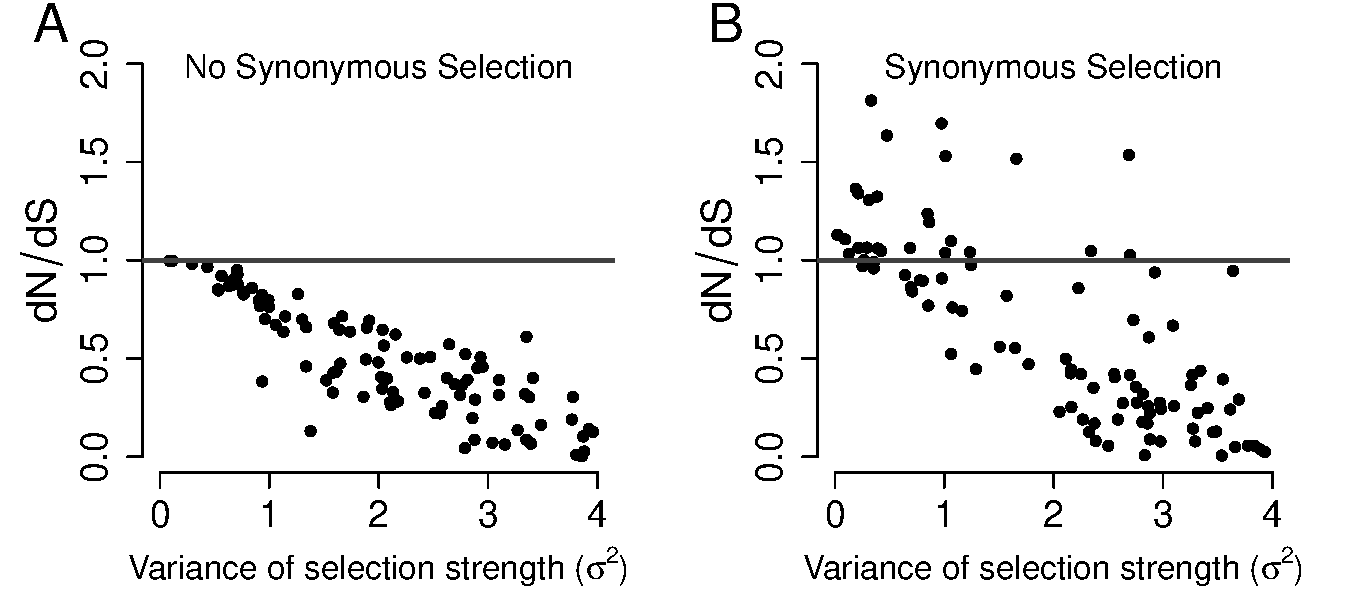
\includegraphics[width=8.7cm]{figures/MainText/dnds_variance.pdf}}
	\caption{\label{dnds_variance} $dN/dS$ decreases in proportion to amino-acid level selection strength. $dN/dS$ is plotted against the $\sigma^2 $ of the simulated distribution of amino-acid scaled selection coefficients. Higher values of $\sigma^2$ indicate larger fitness differences among amino acids, whereas the limiting value of $\sigma^2 = 0$ indicates that all amino acids have the same fitness. (A) Synonymous codons have equal fitness values ($r^2=0.83$). (B) Synonymous codons have different fitness values ($r^2=0.45$). Note that panel B, but not A, shows $dN/dS$ values greater than 1, in spite of the steady-state evolutionary process.}
\end{figure}
		
		
\vspace{2cm}
		
\begin{figure}[htbp]
	\centerline{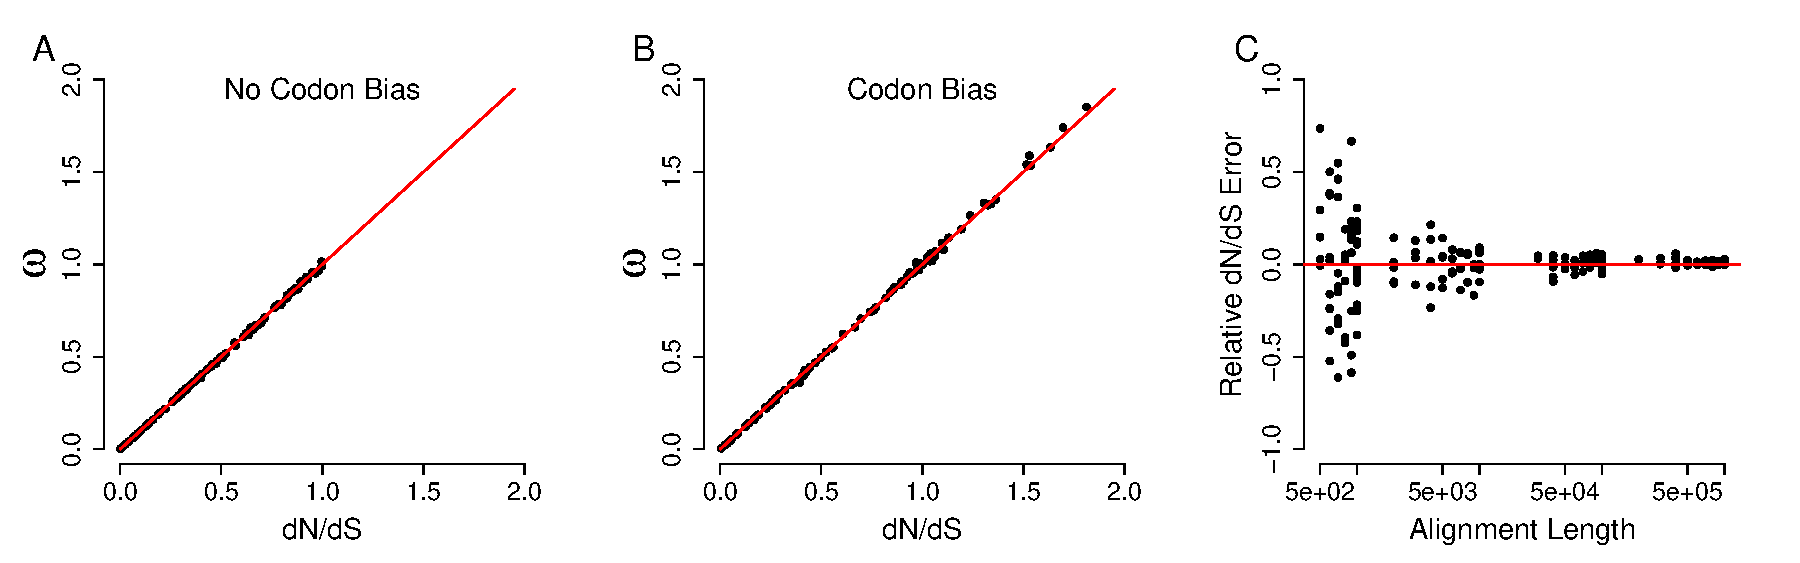
\includegraphics[width=8.7cm]{figures/MainText/regression_convergence.pdf}}
	\caption{\label{reg_conv} Combined modeling approach to assess performance of $dN/dS$ inference frameworks. (A) Protein-coding alignments are simulated in the MutSel modeling framework. $dN/dS$ can then be calculated from scaled selection coefficients as well as through a ML inference framework. Comparing resulting quantities reveals the accuracy in the chosen $dN/dS$ inference framework. (B) Regression between $dN/dS$ values as calculated from scaled selection coefficients and as inferred using the M0 model \cite{GoldmanYang1994,NielsenYang1998,Yangetal2000}. Each point corresponds to a single simulated alignment, and the red line is the $x=y$ line. (C) Convergence of $\omega$ MLEs to the true $dN/dS$ value. The y-axis indicates the relative error of the maximum likelihood $dN/dS$ estimate, and the x-axis indicates the number of positions in the simulated alignment. As the number of positions, and hence the size of the data set, increases, the maximum likelihood estimates converge to the $dN/dS$ values calculated using equations \eqref{eq:pi_i}-\eqref{eq:dS}. The red line is the $y=0$ line, indicating no error.}
\end{figure}
	
\vspace{2cm}
	

\begin{figure}[htbp]
	\centerline{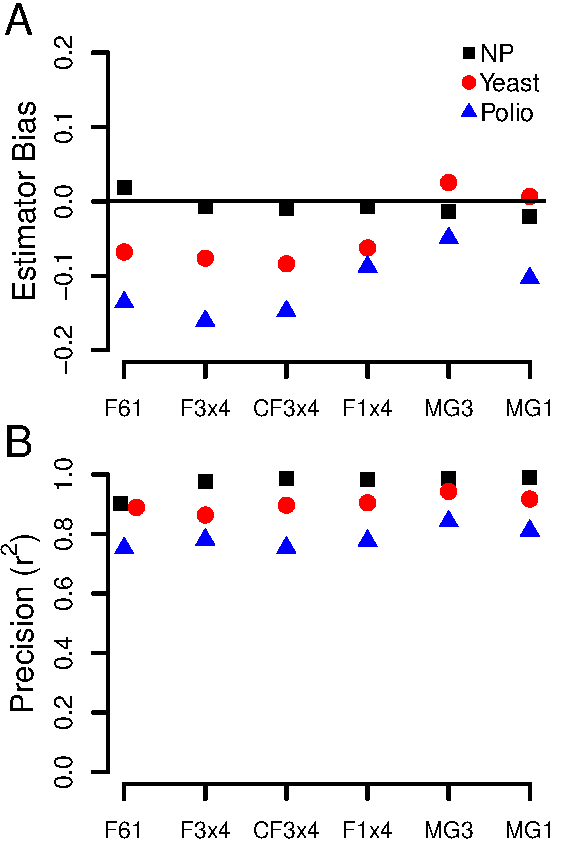
\includegraphics[width=8.7cm]{figures/MainText/nyp_bias_r2.pdf}}
	\caption{\label{nyp_bias_r2} Estimator bias and precision of $\omega$ estimates for various model frequency parameterizations. (A) Estimator bias and (B) $r^2$ values between $dN/dS$ and $\omega$ MLEs across model frequency parameterizations, for each set of nucleotide mutation rates. To calculate bias, we fit a linear model, with $\omega$ as the response and $dN/dS$ as the response, with a fixed slope of 1, and the resulting intercept value is the bias quantity. Negative biases indicate $\omega$ estimates that are, on average, lower than $dN/dS$. For all frequency parameterizations, bias generally increases as mutation rates become increasingly asymmetric. Even so, MG-style models tend to yield far less biased $\omega$ estimates than do GY-style models.}	
\end{figure}

\vspace{2cm}


\begin{table}[htbp]
	\caption {\label{tab:dAIC} Mean $\Delta$AIC for datasets simulated with NP, Yeast, or Polio mutation rates.}
	\begin{tabular}{l c c c}
		\hline\noalign{\smallskip}
		\multicolumn{1}{c}{Frequencies} & NP & Yeast & Polio \\
		\noalign{\smallskip}\hline\noalign{\smallskip}
		F61 & 0 & 0 & 0 \\ 
		CF3x4 & -9627.5 & -7951.8 & -7975.9 \\ 
		MG1 & -13325.5 & -10042.0 & -5147.6 \\ 
		F1x4 & -13524.5 & -13658.5 & -15468.3 \\ 
		MG3 & -14401.3 & -12851.6 & -8624.9 \\ 
		F3x4 & -14807.2 & -17385.3 & -19384.6 \\ 
		\noalign{\smallskip}\hline\noalign{\smallskip} 
	\end{tabular}
	Based on AIC scores, the F61 parameterization strongly outperforms all other model parameterizations for all mutation rates, even so the F61 framework yields neither the most accurate nor the most precise parameter estimate. Note that the order of frequency models shown in the table corresponds to the model ranking for NP, and the ranking differs somewhat for yeast and polio datasets. AIC is computed as $AIC = 2(k - \ln(L))$, where $k$ is the number of free parameters of the model, and $\ln(L)$ is the log-likelihood. As codon and/or nucleotide frequency parameters are directly estimated from the data, all models have 3 free parameters ($\omega$, $\kappa$, and a global branch length scaling parameter).
\end{table}

\vspace{2cm}


\begin{figure}[htbp]
	\centerline{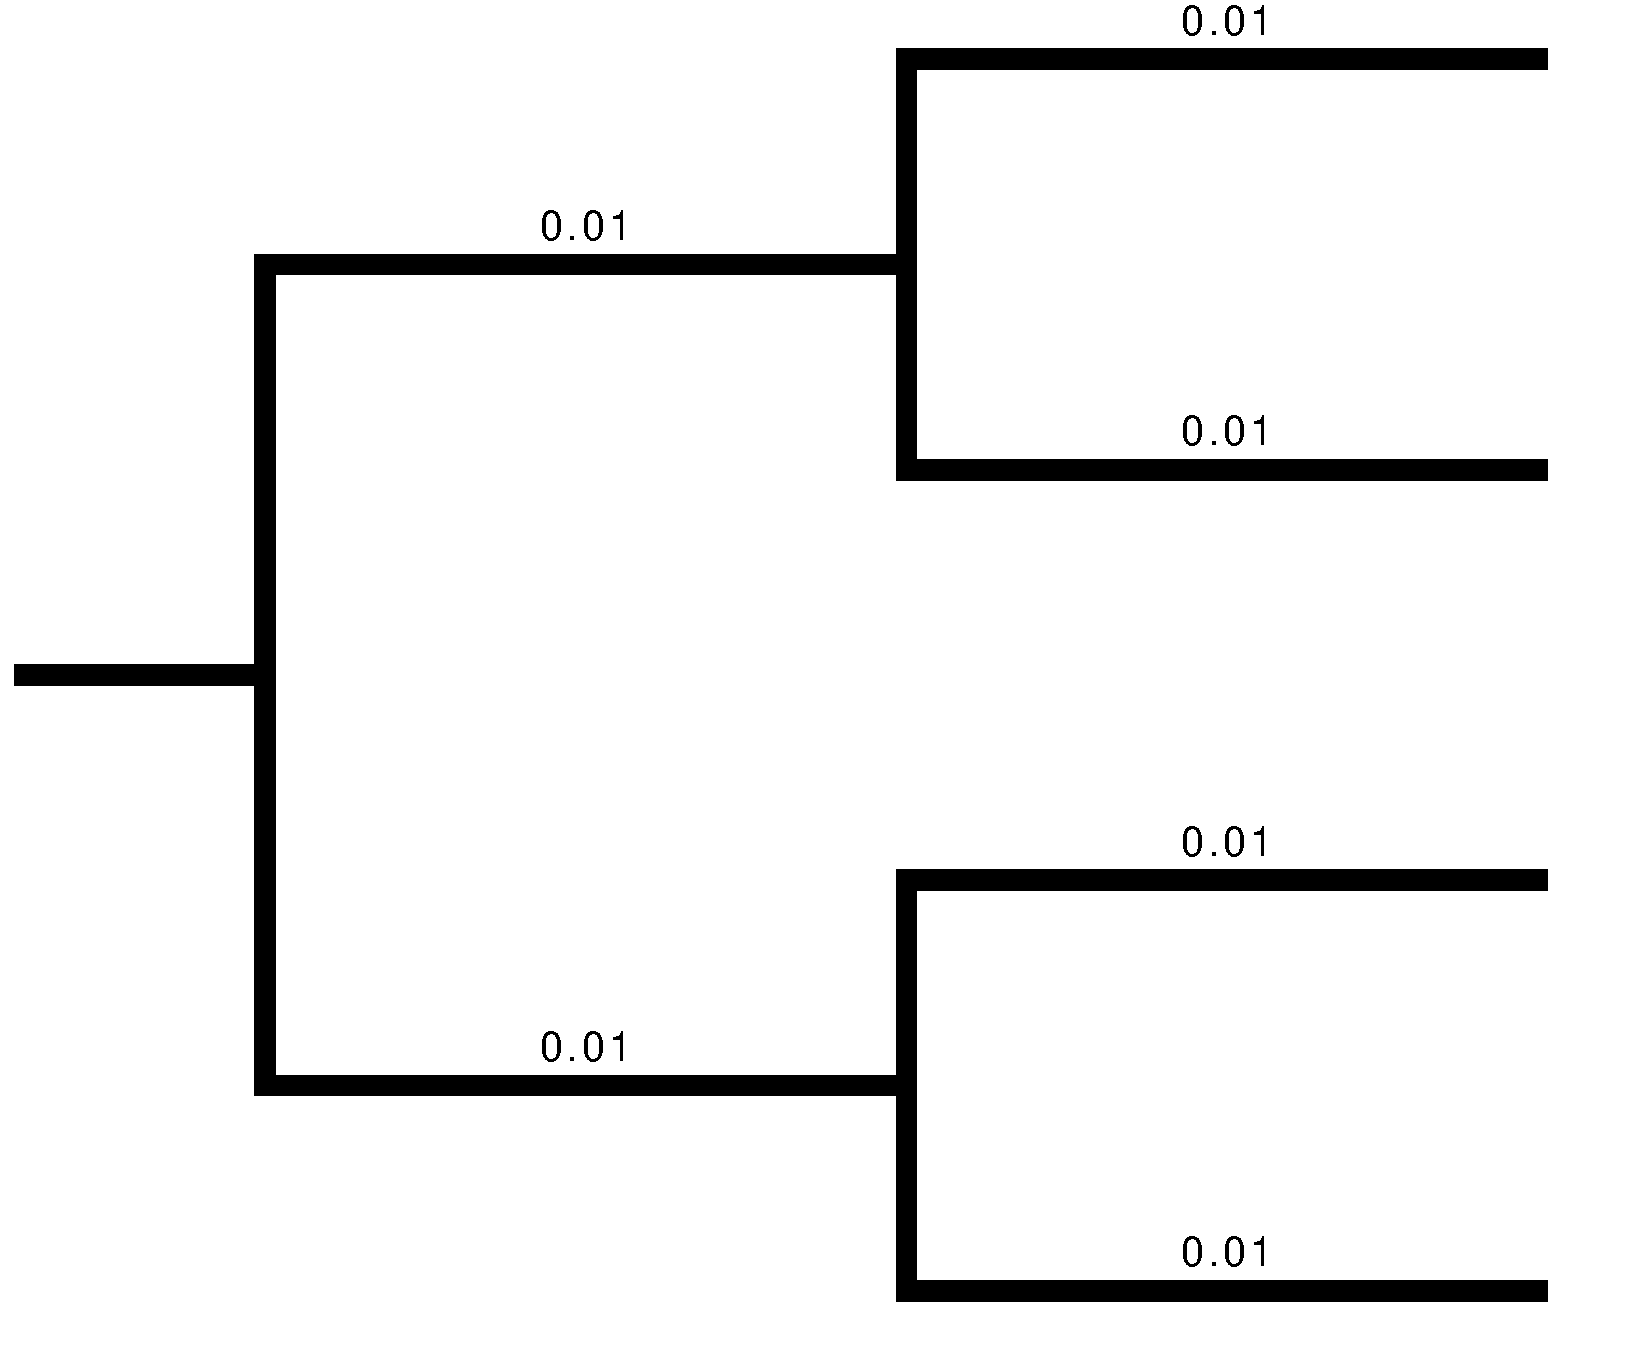
\includegraphics[width=6cm]{figures/MainText/simtree.pdf}}
	\caption{\label{tree} Phylogeny used for all simulated alignments.}	
\end{figure}


\clearpage

	
\section*{Supplementary Information}

\vspace{2cm}

\noindent Table S1. Estimator bias of $\omega$ MLEs and the true $dN/dS$ values, for all nucleotide mutation rates and model frequency parameterizations examined. Negative bias values indicate that $\omega$ MLEs are, on average, lower than $dN/dS$. All biases are statistically significant (different from 0), with all $P < 2\times10^{-16}$ except for the estimator bias associated with yeast mutation rates for MG3, where $P = 5.4\times10^{-5}$.
\begin{table}[htbp]
	\begin{tabular}{c c c c c c c}
		\hline\noalign{\smallskip}
		Mutation rate & MG1 & F1x4 & MG3 & CF3x4 & F3x4 & F61 \\
		\hline\noalign{\smallskip}
		NP & -0.014 & -0.02 & -0.007 & -0.009 & -0.007 & 0.019 \\ 
		Yeast & 0.025 & 0.007 & -0.063 & -0.084 & -0.076 & -0.068 \\ 
		Polio & -0.049 & -0.103 & -0.088 & -0.148 & -0.161 & -0.136 \\ 
		\noalign{\smallskip}\hline\noalign{\smallskip}
	\end{tabular}
\end{table}	


\vspace{2cm}

\noindent Table S2. Precision, measured as the squared correlation coefficient $r^2$, of $\omega$ MLEs relative to the true $dN/dS$ values, for all nucleotide mutation rates and model frequency parameterizations examined. All values shown are statistically significant, with all $P < 2\times10^{-16}$ .
\begin{table}[htbp]
	\begin{tabular}{c c c c c c c}
		\hline\noalign{\smallskip}
		Mutation rate & MG1 & F1x4 & MG3 & CF3x4 & F3x4 & F61 \\
		\hline\noalign{\smallskip}
		NP & 0.988 & 0.989 & 0.985 & 0.986 & 0.977 & 0.902 \\ 
		Yeast & 0.943 & 0.917 & 0.905 & 0.897 & 0.864 & 0.889 \\ 
		Polio & 0.842 & 0.811 & 0.777 & 0.754 & 0.781 & 0.752 \\ 
		\noalign{\smallskip}\hline\noalign{\smallskip}
	\end{tabular}
\end{table}	

\newpage

\begin{landscape}
	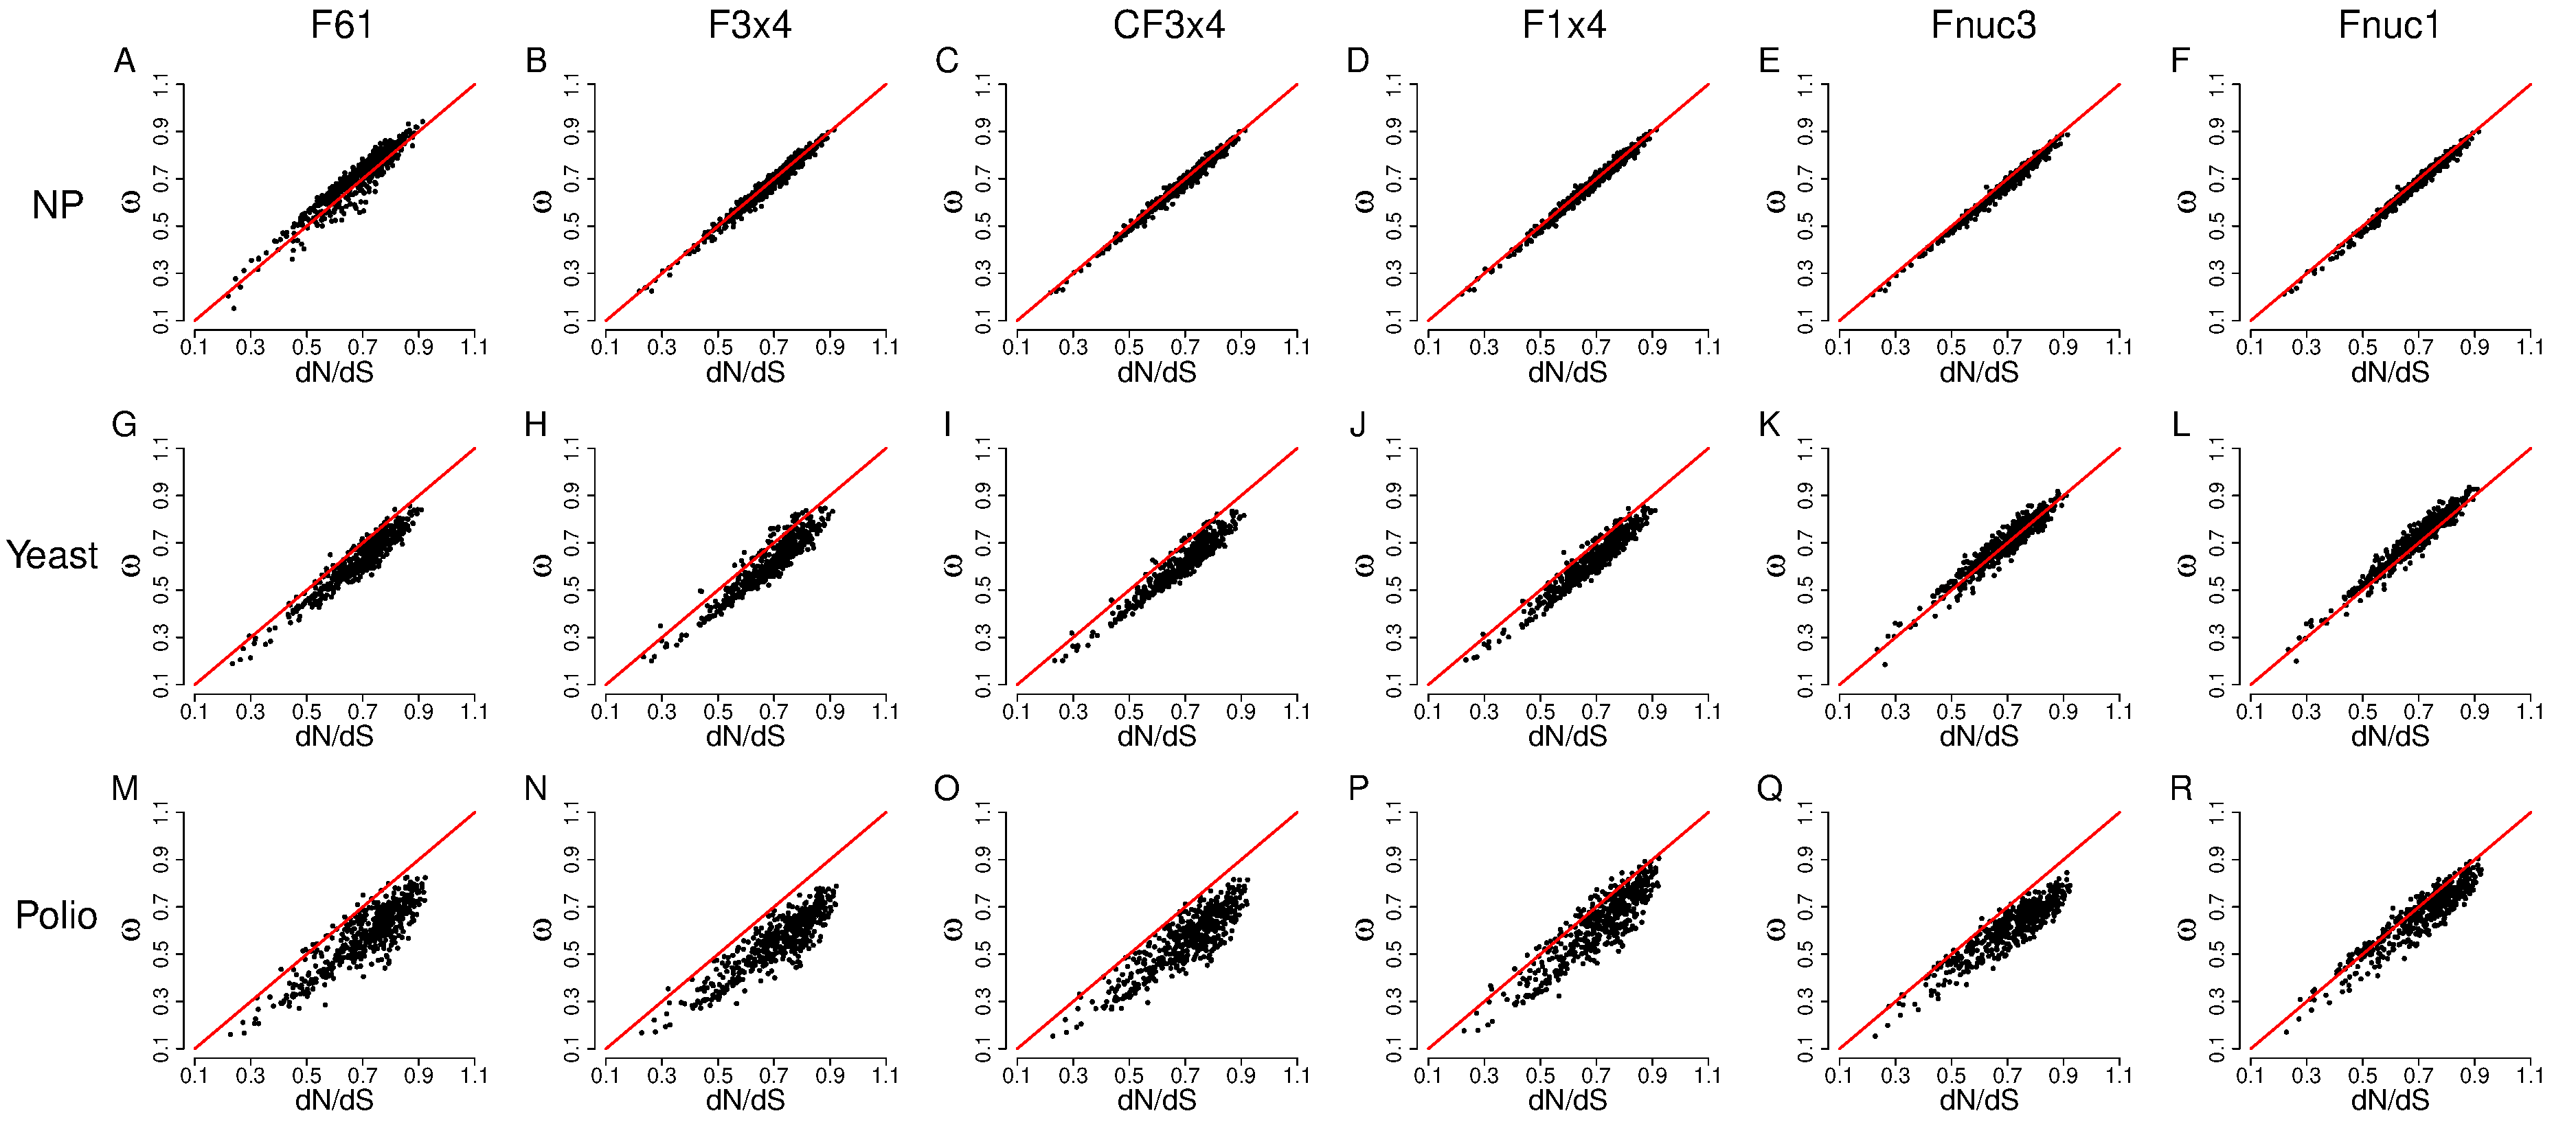
\includegraphics[width=9.5in]{figures/SI/nyp_regression.pdf}
	\vspace{0.5cm}
	
	Figure S1. Regressions for inferred $\omega$ estimates and $dN/dS$ values, as calculated from scaled selection coefficients, for datasets simulated using experimental fitnesses and mutation rates. Each point represents an alignment, and red lines are the $x=y$ line.
\end{landscape}



\end{document}

